% P05 benchmark paired scatter; aggregate station-instrument domain means.
% Each point is a domain mean over common complete outer contexts; not an independent sample.
% data_sha256=235e8a7e1a4b0fc17b736ee7db3dcb16eaac30e233bc9eeb9ab4d033958dcc67
\documentclass[tikz,border=5pt]{standalone}
\ifdefined\pdfinfoomitdate\pdfinfoomitdate=1\fi
\ifdefined\pdfsuppressptexinfo\pdfsuppressptexinfo=-1\fi
\ifdefined\pdftrailerid\pdftrailerid{}\fi
\usepackage{pgfplots}
\usepgfplotslibrary{groupplots}
\pgfplotsset{compat=1.18}
\definecolor{p05Blue}{HTML}{0072B2}
\definecolor{p05Orange}{HTML}{E69F00}
\definecolor{p05Purple}{HTML}{CC79A7}
\begin{document}
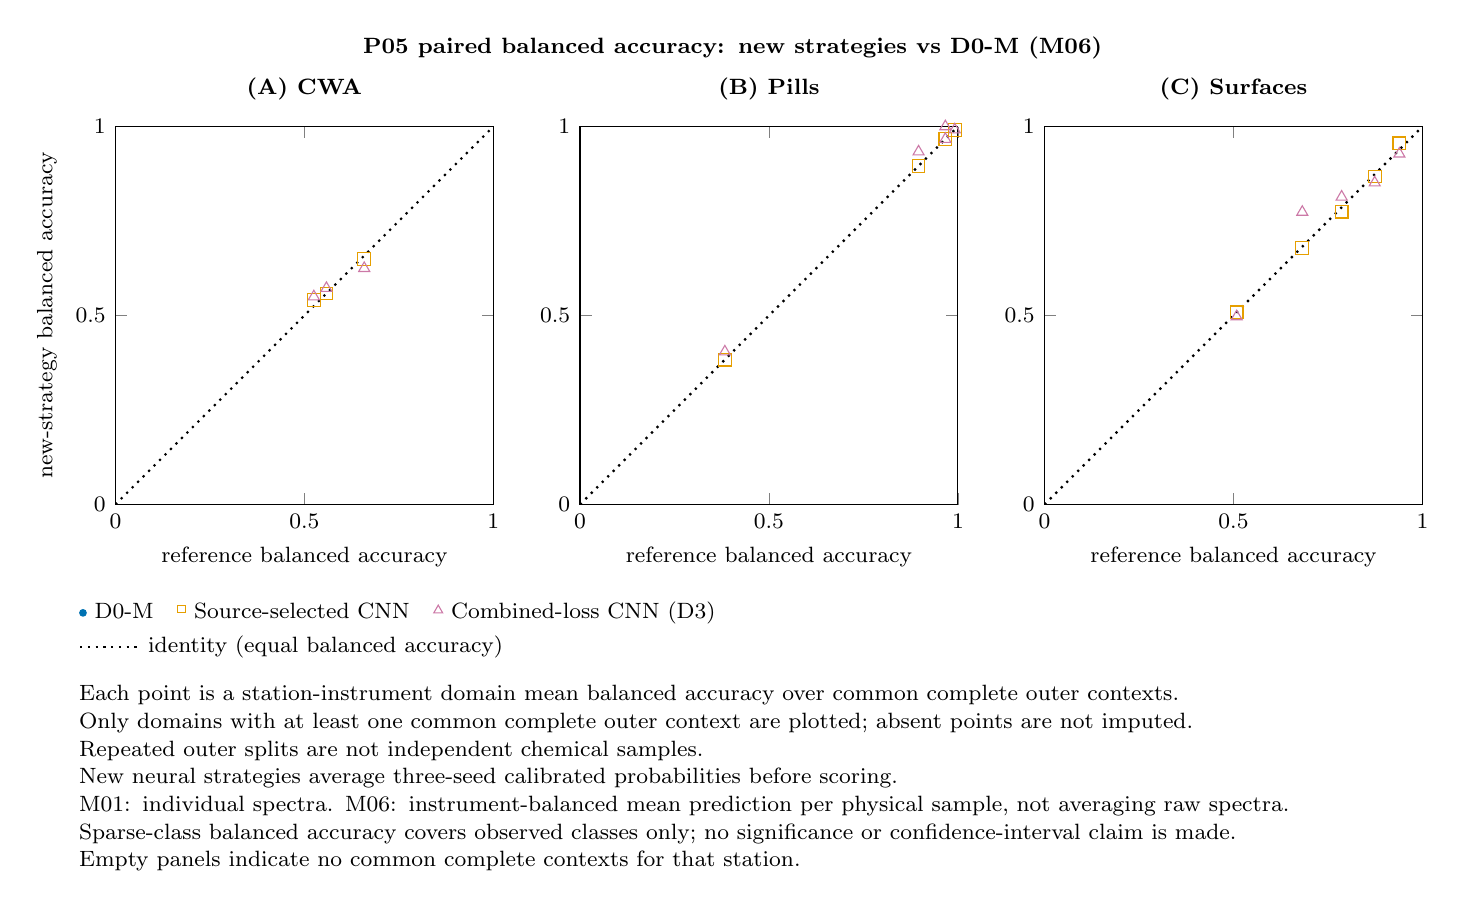
\begin{tikzpicture}
\begin{groupplot}[
  group style={group size=3 by 1, horizontal sep=1.1cm},
  width=4.8cm, height=4.8cm, scale only axis,
  xmin=0, xmax=1, ymin=0, ymax=1,
  xtick={0,0.5,1}, ytick={0,0.5,1},
  tick label style={font=\fontsize{8}{10}\selectfont, color=black},
  label style={font=\fontsize{8}{10}\selectfont, color=black},
  title style={font=\fontsize{8}{10}\selectfont\bfseries, color=black},
]
\nextgroupplot[title={(A) CWA}, xlabel={reference balanced accuracy}, ylabel={new-strategy balanced accuracy}]
\addplot[only marks, mark=square, mark size=2.3pt, color=p05Orange, mark options={fill=none, draw=p05Orange}] coordinates {(0.52499999999999991,0.54166666666666663) (0.55833333333333335,0.55833333333333335) (0.65833333333333344,0.65000000000000002)};
\addplot[only marks, mark=triangle, mark size=2.3pt, color=p05Purple, mark options={fill=none, draw=p05Purple}] coordinates {(0.52499999999999991,0.54999999999999993) (0.55833333333333335,0.57222222222222219) (0.65833333333333344,0.62499999999999989)};
\addplot[black, dotted, line width=0.8pt] coordinates {(0,0) (1,1)};
\nextgroupplot[title={(B) Pills}, xlabel={reference balanced accuracy}]
\addplot[only marks, mark=square, mark size=2.3pt, color=p05Orange, mark options={fill=none, draw=p05Orange}] coordinates {(0.89583333333333326,0.89583333333333326) (0.96666666666666656,0.96666666666666656) (0.38333333333333325,0.38333333333333325) (0.96666666666666656,0.96666666666666656) (0.99166666666666681,0.99166666666666681)};
\addplot[only marks, mark=triangle, mark size=2.3pt, color=p05Purple, mark options={fill=none, draw=p05Purple}] coordinates {(0.89583333333333326,0.93333333333333335) (0.96666666666666656,0.96666666666666656) (0.38333333333333325,0.40416666666666662) (0.96666666666666656,1) (0.99166666666666681,0.99166666666666681)};
\addplot[black, dotted, line width=0.8pt] coordinates {(0,0) (1,1)};
\nextgroupplot[title={(C) Surfaces}, xlabel={reference balanced accuracy}]
\addplot[only marks, mark=square, mark size=2.3pt, color=p05Orange, mark options={fill=none, draw=p05Orange}] coordinates {(0.5083333333333333,0.5083333333333333) (0.68194444444444435,0.67916666666666659) (0.93888888888888888,0.95555555555555549) (0.87361111111111123,0.86805555555555558) (0.78611111111111109,0.77500000000000002)};
\addplot[only marks, mark=triangle, mark size=2.3pt, color=p05Purple, mark options={fill=none, draw=p05Purple}] coordinates {(0.5083333333333333,0.49722222222222212) (0.68194444444444435,0.77361111111111103) (0.93888888888888888,0.92777777777777781) (0.87361111111111123,0.85138888888888897) (0.78611111111111109,0.81388888888888877)};
\addplot[black, dotted, line width=0.8pt] coordinates {(0,0) (1,1)};
\end{groupplot}
\node[anchor=south, font=\fontsize{8}{10}\selectfont\bfseries, color=black, align=center, text width=16.6cm] at (current bounding box.north) {P05 paired balanced accuracy: new strategies vs D0-M (M06)};
\node[anchor=north, font=\fontsize{8}{10}\selectfont, color=black, align=left, text width=16.6cm] (p05legend) at ([yshift=-2mm]current bounding box.south) {\tikz[baseline=-0.6ex]\fill[p05Blue](0,0)circle(1.4pt);\ D0-M\quad \tikz[baseline=-0.6ex]\draw[p05Orange](0,0)rectangle(2.8pt,2.8pt);\ Source-selected CNN\quad \tikz[baseline=-0.6ex]\draw[p05Purple](0,0)--(1.6pt,2.8pt)--(3.2pt,0)--cycle;\ Combined-loss CNN (D3)\\[0.8mm]\tikz[baseline=-0.6ex]\draw[black,dotted,line width=0.8pt](0,0)--(0.75,0);\ identity (equal balanced accuracy)};
\node[anchor=north, font=\fontsize{8}{10}\selectfont, color=black, align=left, text width=16.6cm] at ([yshift=-1mm]p05legend.south) {Each point is a station-instrument domain mean balanced accuracy over common complete outer contexts.\\Only domains with at least one common complete outer context are plotted; absent points are not imputed.\\Repeated outer splits are not independent chemical samples.\\New neural strategies average three-seed calibrated probabilities before scoring.\\M01: individual spectra. M06: instrument-balanced mean prediction per physical sample, not averaging raw spectra.\\Sparse-class balanced accuracy covers observed classes only; no significance or confidence-interval claim is made.\\Empty panels indicate no common complete contexts for that station.};
\end{tikzpicture}
\end{document}
